\chapter{Implementation}

This chapter describes details, problems and limitations of the thesis implementation part.

The implementation of the prototype is divided into three main parts: compression, streaming and rendering.
The compression is implemented as a standalone Java application, which compresses BTFs from the Bonn University \cite{btfBonn}.
It is possible to adapt any other BTF databases for our prototype by resampling the BTFs \cite{resampling}.
For the streaming server implementation Node.js \cite{nodejs} is used.
The client side 3D rendering is done using XML3D \cite{xml3d}, a declarative 3D approach that integrates 3D graphics into the DOM.
An overview of the architecture of prototype is depicted in Figure \ref{fig:overview}.

\begin{figure}[h]
 \centering
 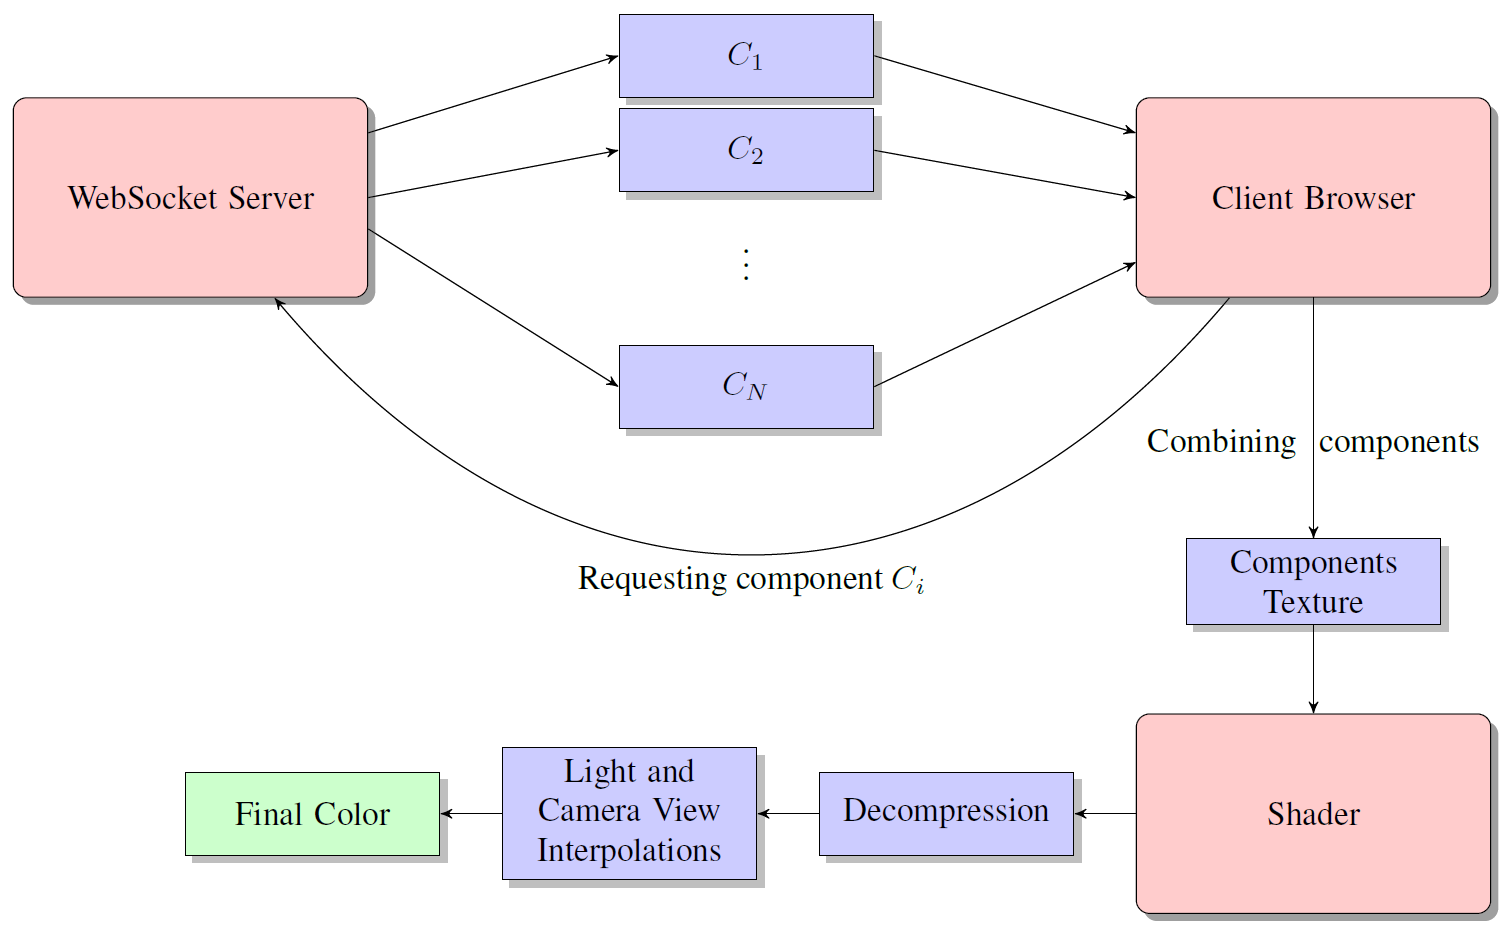
\includegraphics[width=1.0\textwidth]{figures/overview}
 \caption[Model Overview ] {
 	{\bf Model Overview}

	
	}
 \label{fig:overview}
\end{figure}



\section{Compression}
\label{section:impl_compression}

The implementation of the singular value decomposition (SVD) is the main part of the PCA implementation.
 We use \emph{jblas} \cite{jblas} developed by Mikio Braun,
 is a BLAS (Basic Linear Algebra Subprograms) implementation for Java.
 
 
The compressed BTFs  have to be sent to the shader. 
  OpenGL Shading Language (GLSL) version 1.0 supports uniform arrays, however, they do not fully support dynamic indexing  \cite{glsl}.
Fortunately, it is possible to transform arrays of data into textures. 
After performing SVD, the matrices $U$, $\Sigma$, $V$ are saved as PNG images. (See Chapter \ref{chapter:implementation}).
Values of matrices $U$ and $V$ are in the range of $[-1;1]$.
 Those values have to be mapped to the image domain, i.e. $[0;1]$.

 Each component of the matrix $U$ is stored as a separate PNG image.
 For example, if compressed BTF data has $C$ principal components, then this would result in $C$ separate images.
 This is done for streaming purposes, to transfer each component one by one from the server to the client.
 We use  RGBA color space to save four components into the one pixel, because it is possible to do efficient multiplication in the shader by using vector multiplications.
Matrices $V$ and $\Sigma$ are saved in the single shared texture, as they are small in size.

 The matrix $\Sigma$ is a diagonal matrix.
 The values of $\Sigma$ can be bigger than the image color value, i.e. an 8-bit value.
 In practice the values of $\Sigma$ for Bonn University BTFs \cite{btfBonn} are not bigger than a four digit number $a_{4}a_{3}a_{2}a_{1}$.
We split the value into two values, i.e. 
 
{\centering$ \underbrace{a_{4}a_{3}}_{R} \underbrace{a_{2}a_{1}}_{G}$\\}
 
It means that two values of $\Sigma$ are mapped into the one pixel, i.e.  one value to RG  channels and the second to BA channels.
If the value of  $\Sigma$ exceed the four digit number, then it is possible to adapt this technique further in a similar manner.


We noticed that for BTFs from the Bonn Database \cite{btfBonn} the \emph{jblas} \cite{jblas} library produces relatively sparse values for $U$ and $V$, i.e. close to zero.
 Due to floating point imprecisions this sparsity results in decompression errors.
 To compensate for this precision limitation we scale the values of the matrices $U$ and $V$.
 This improves the overall decompression error by  approximately $5\%$.
 The scaling factor is determined by the following equation:
 
 {\centering$ factor(M)=10^{floor(min[log10(min(M)),log10(max(M)]))}$ \\}
 
 where M is the matrix $U$ or $V$. The term $floor(min[log10(min(M)),log10(max(M))])$ calculates the degree with which it is possible to multiply the matrix and preserve the original values range, i.e. $[-1;1]$.
 If it is not possible, the resulting factor will be $1$.
As the decompression is computed as multiplication of $U\Sigma V$, we have to remain the original decompressed BTF values.
We do this by  multiplying all $\Sigma$ values by the factor $\tfrac{1}{factor(M)}$ if we scale either $U$ or $V$.


 
\section{Streaming}
\label{section:impl_streaming}

When rendering BTFs in a web-browser, all data has to be transferred before rendering.
Even compressed BTF data can be tens of megabytes in size and can take a considerable amount of time for transmission.
We propose to stream the BTF data to reduce the latency before rendering can start.
 The user will be able to see a low quality preview of the original BTF in just a few seconds. 
In our case, principal components are streamed one by one using WebSockets \cite{WebSockets}.
Each principal component covers the full angular domain, so that the BTF can be rendered for any camera and light direction at any time during the streaming process.
The rendering quality is enhanced whenever a new component arrives.


 WebSockets are an efficient way for real-time client server communication.
 They are widely supported by desktop as well as mobile browsers.
WebSockets have several advantages over HTTP Polling, Long Polling, Streaming approaches \cite[Ch.\ 1]{WebSockets}.  
As they provide a Full-Duplex connection, the client and the server can reuse the same connection for communication.
In contrast Polling requires the client to regularly check for new information.
 This single connection dramatically reduces the latency.
HTTP Streaming also uses a single connection, but only from the server to the client and is currently only available for ascii  data. 
Firewalls may additionally buffer the HTTP response, which can result in increased latency.
All in all WebSockets save bandwidth, CPU time and reduce  latency compared to HTTP streaming or polling approaches.

We use Node.js \cite{nodejs} as a server side platform, which enables realtime streaming using WebSockets. 
On the client side we use Xflow \cite{xflow}, a declarative data flow processing language integrated into XML3D \cite{xml3d}.
 Xflow is used to gather and store all already transferred principal components in a texture. (See Chapter  \ref{section:decompression}).





Consider Figure \ref{fig:overview} that depicts how the streaming works on practice.
When the user connects to the streaming server and the HTML page loads completely, 
i.e. the 3D object is on the client side, the JavaScript client side sends the message to the Node.js server to start streaming the BTF data.
All the compressed BTFs are located on the Node.js server.
At the start of the stream, we first send texture $R$ and meta data. (See Chapter  \ref{section:decompression}).
Afterwards, indiviual principal components $C_{i}$ are streamed in chunks one by one as PNG images.
Each principal component $C_{i}$ covers all the angular domain of the BTF, i.e. all possible camera and light directions.

Received PNG images are decoded and stored into the texture $L$. (See Chapter  \ref{section:decompression}).
This update in turn refreshes the rendering.
Even with the first principal component the resulted rendering looks plausible.
With further components the overall quality of the image improves, i.e. specularities are increasing and small micro-structures become more visible.


Because JavaScript is single threaded every time the principle components are assembled into the texture $L$ the framerate and responsiveness of the overall application is affected.
This could be fixed by sending each  principal component as an individual textures to the shader.
However, the number of textures are limited by the specifications of the GPU.
Also, we did not test streaming of multiple BTFs, i.e. if there are several 3D objects in one scene that request BTFs at the same time.
 Our current implementation of streaming does not support this, but this could be included in the future.
 
 
\section{Rendering}
\label{section:impl_rendering}


We use XML3D \cite{xml3d} to embed 3D graphics into the HTML page. XML3D allows for a declarative description of the 3D scene.
The XML3D polyfill uses WebGL for rendering and enables the user to define custom GLSL shaders.

The shader design is depicted in Figure \ref{fig:shader}.
The compressed BTF data is accessed in the shader in the form of two textures. 
The first texture $L$ stores principal components and the second $R$ stores PCA weights. (See Chapter \ref{section:decompression}).
First, we find the three closest directions for the camera and light directions. (See Chapter \ref{chapter:finding_triangle}).
Then, we compute barycentric coordinates for interpolation as described in Chapter \ref{chapter:barycentric}.

\begin{figure}[h]
 \centering
 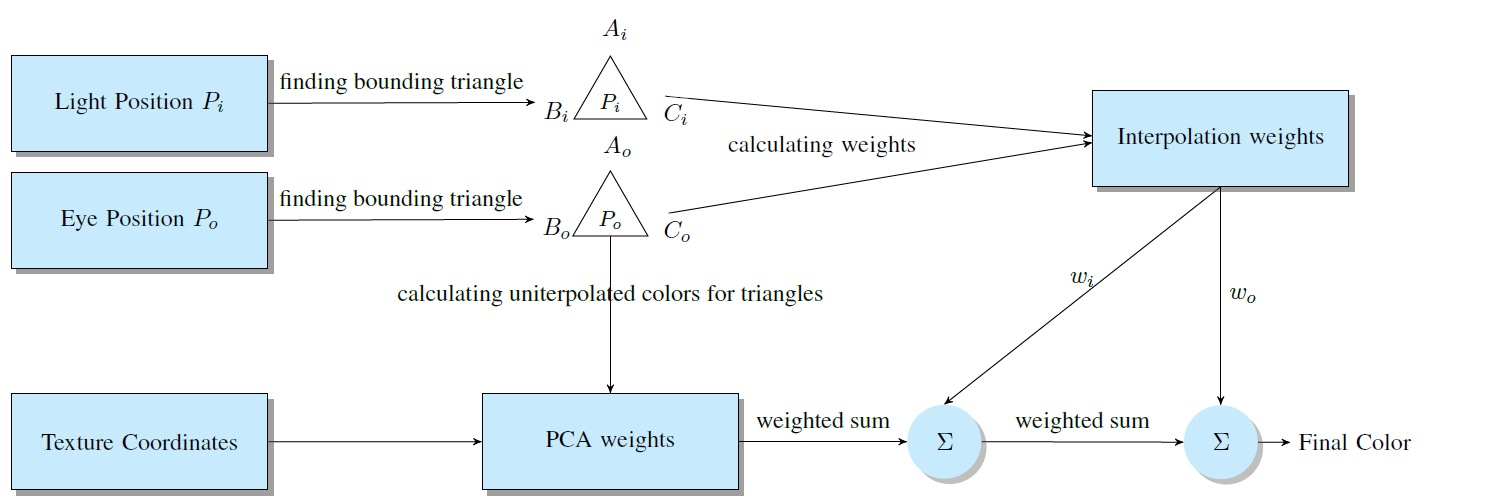
\includegraphics[width=1.0\textwidth]{figures/shader}
 \caption[Shader Design] {
 	{\bf Shader Design }

 }
 \label{fig:shader}
\end{figure}


In the next step we sample the input textures to decompress the needed values for the found closest directions.
We have three closest directions per camera and light directions. This means for the interpolation we need to have nine color values. 
For a given texture coordinates $u,v$ we lookup the index of the first principal component, with which it will be possible to start the decompressing.
All the principal components are written linearly in texture $L$, i.e. one by one. 
We have the following mapping to get the needed index:

{\centering$indexL(i,j)= (b*N^2+ (i*N+j))*C$ \\}

where $i=\left \lfloor u*N\right \rfloor$, $j=\left \lfloor v*(N) \right \rfloor$, $b$ is the number of subsets, $N$ is the dimension of the compressed image and $C$ is number of components.
The parameter $b$ depends on the number of subsets on which PCA is separately done. (See Chapter \ref{section:algorithm_step}).

Texture $R$ stores PCA weights.
The mapping depends on the camera direction $v=(\theta_v,\phi_v)$ and light direction $l=(\theta_l,\phi_l)$.
 It is defined as:

{\centering$ indexR(v,l)=offset(\theta_v,\phi_v)+offset(\theta_l,\phi_l)$\\}

where  $offset(\theta,\phi)=(\tfrac{\theta}{\Delta\theta}+\tfrac{\phi}{\Delta\phi})$, where $\Delta\theta$ and $\Delta\phi$ are quantization step sizes.

When all the indices are computed and textures L and R can be sampled, we decompress the colors as defined in Chapter \ref{section:decompression}.


In a final step we combine nine decompressed colors and the early found interpolation weights to get the final color. (See Chapter \ref{chapter:interp_algo}).

The implemented shader has some limitations. First of all, the number of principal components has to be fixed and known beforehand, because GLSL version 1.0 does not support dynamic looping \cite{glsl}.
Secondly, the number of principal components are bound by the maximum dimensions a GPU allows for the texture $L$.
This problem could be fixed using multiple textures. However, the number of possible active textures is limited, too.






 



